\subsection{Sector indicators}

From the \co data we predicted for 2020 without considering COVID-19, we now want to deduce actual \co for this year. As monthly \co emission data is not available, we needed to find a way to model the emissions during the lock-down.
\co emissions can be split up in five major sectors, as depicted in \autoref{tab:sector_contributions}. For each sector, we know the yearly behavior but not the monthly. In this section, we will focus on finding monthly data for each sector.

\begin{table}[h!]%todo: Pie chart?, Values add up to 109 \% sadly
	\centering
	\begin{tabular}{lr}
		\hline
		Sector & Contribution to total emissions in 2018\\
		\hline
		\hline
		Power industry &  \(39.42\%\)\\ 
		Buildings &   \(10.90\%\)\\ 
		Mobility &   \(23.92\%\)\\ 
		Other industrial combustion &   \(22.30\%\)\\ 
		Other sectors &   \(12.56\%\)\\ 
		\hline &\\
	\end{tabular}
	\caption{All five majors sectors  and their contributions to the total \co emissions. Calculated from the EDGAR dataset.}%todo: source
	\label{tab:sector_contributions}	
\end{table}	



Knowing each sectors usual contribution to the total emissions, we want to find the behavior of the \co emissions of each sector during the lock-down. To do so, we use monthly data available to us that can be seen as an indicator for the respective sector. For each country, we extract one value per month in 2020 that we apply to our estimated 2020 \co emission data without considering COVID-19. In conclusion, we modulate our yearly data with monthly values to obtain monthly \co emission data for 2020.

\subsubsection{Power Industry}
The classification by sectors is given by the report of EDGAR \cite{crippa2019fossil}. The emissions produced by this sector refer to power and heat generation plants (public \& autoproducers). In a general view, it is the main source of greenhouse gas emissions. The original data from this sector is until 2018 and annual, so we cannot appreciate the impact of COVID-19. We decided to explore some indicators which were monthly updated to get an intuition. 


\paragraph{Indicators}
\begin{itemize}
	\item \textbf{Natural gas prices:} \cite{gas} dataset contains monthly and daily prices of natural gas, starting from January 1997 to current year. Prices are in nominal dollars.
	\item \textbf{Brent spot prices:} \cite{brent} Europe Brent and WTI (Western Texas Intermediate) Spot Prices (Annual/ Monthly/ Weekly/ Daily) from EIA U.S. (Energy Information Administration).
	\item \textbf{Electricity, gas, steam and air conditioning supply:} \cite{production} industry production per European country.
	\item \textbf{Supply oil:} \cite{production} as the previous reference, it is defined also per European country.
\end{itemize}

\paragraph{Strategy}
Due to the lack of monthly emission data for this sector which could show us the impact of COVID-19, we had to based our predictions in these indicators.

The first approach was to modulate the annual emissions with an indicator, in order to get monthly resolution. We could get the weights for each month in the indicator and apply it to the emissions. Then, we could apply machine learning to predict the emissions using indicators, what would be our data considering COVID-19 against the time series prediction of the emissions which represents the data without considering COVID-19. The problem is we were using twice the same data (an indicator), first to modulate the emissions and then to train the model.

For this reason we chose to change the strategy. Now the procedure was to find the most correlated indicator per each country between these four (consider that for non European countries we only have the natural gas and brent prices). Then, we assume the emissions behave as the selected indicator and we are able to identify if there is any change, comparing the real values of the indicator with a time series prediction from previous months affected by COVID-19. The steps are the following:

\begin{enumerate}
	\item \textbf{Selection of most correlated indicator:} we looked for only one indicator per country which could explain the behavior of the emissions. 
	\item \textbf{Time series prediction from december of 2019:} we predict the last months when the COVID-19 had not a big impact, in order to have a reference to compare. The prediction was using the SARIMA model \cite{sarima}. 
	\item \textbf{Extracting COVID-19 influence:} as we have current data from the last months (from January to May of 2020), we can observe a relative change respect the predicted values.
\end{enumerate}


\paragraph{Results}
Depending on the country we are studying, the obtained correlation is very different. 

In Figure \ref{fig:indicators_EEUU_China} we have two cases with only two indicators: United States and China. In the first one we got a correlation larger than 0.8, while in China it does not reach 0.1.
\begin{figure}[h!]
	\centering
	\subfloat[United States]{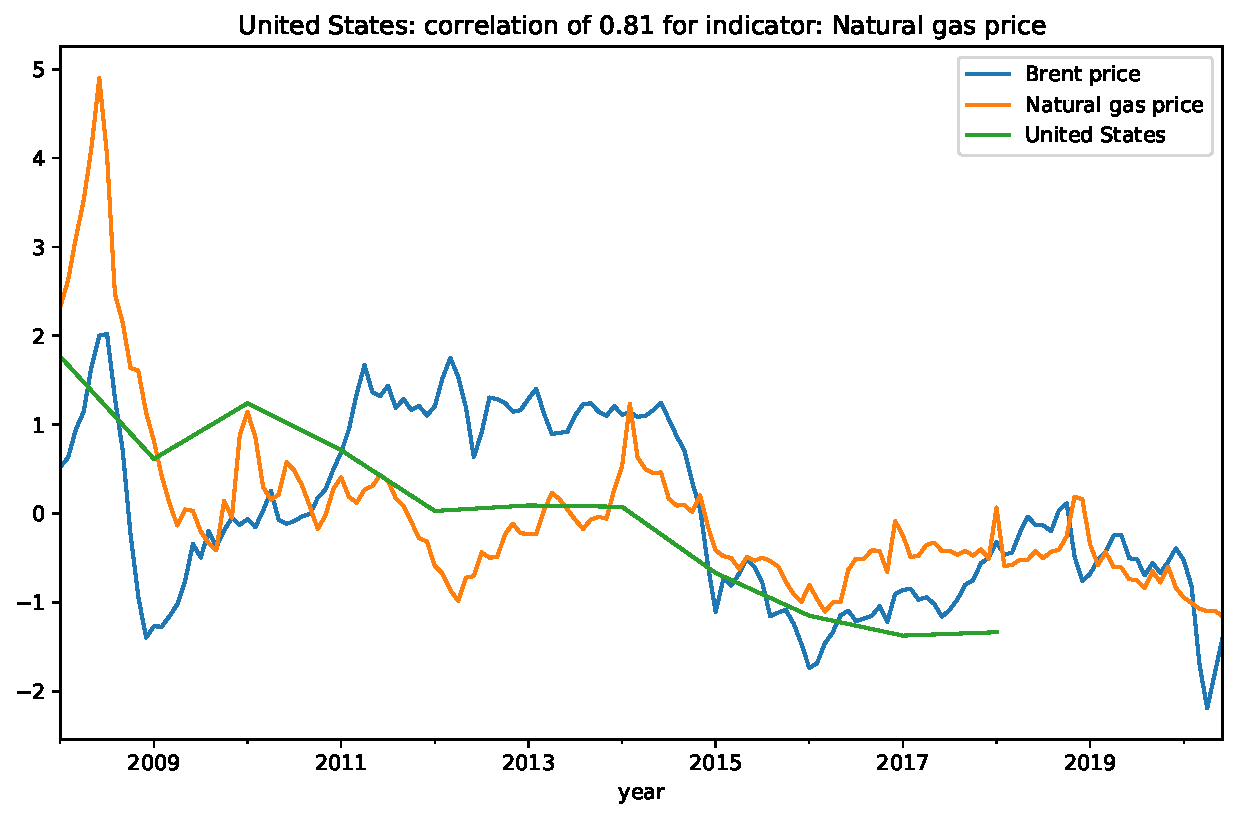
\includegraphics[width=0.5\linewidth]{../power_industry/United States_indicators}}
	\subfloat[China]{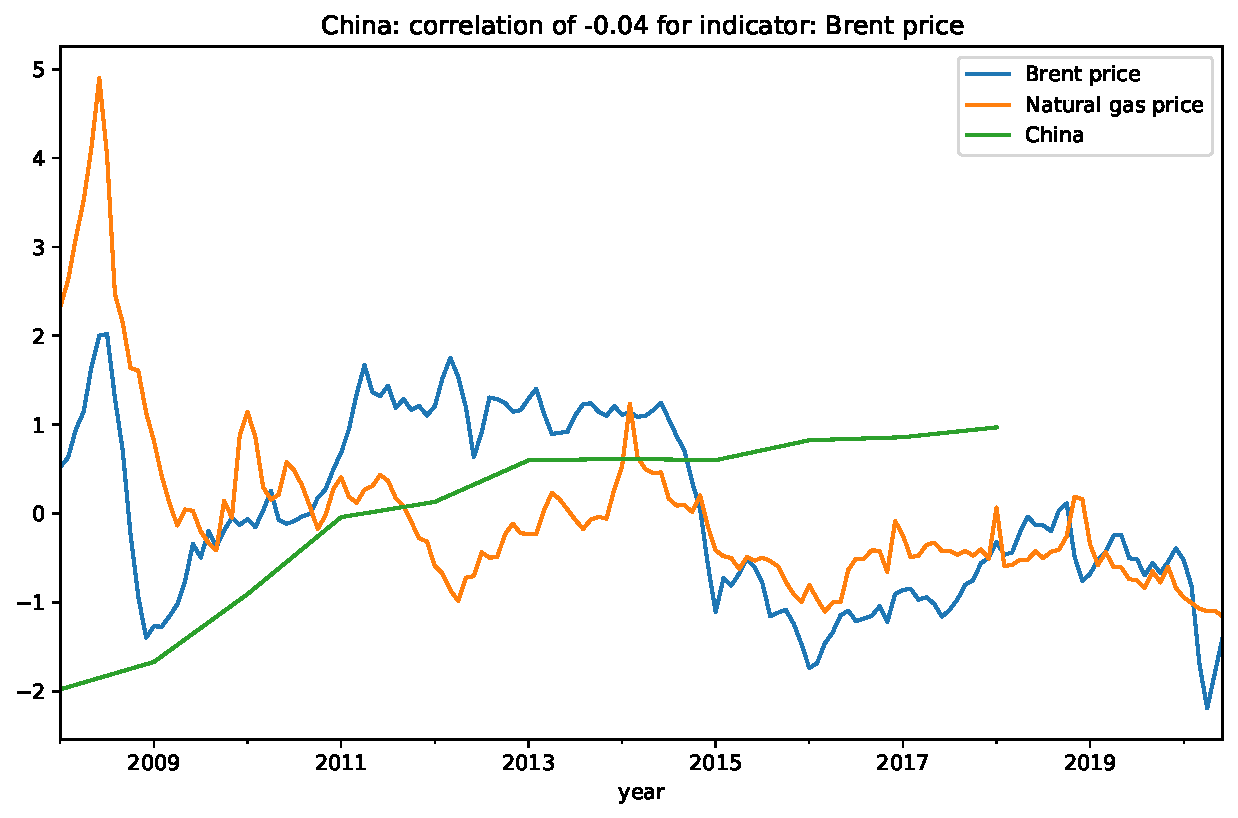
\includegraphics[width=0.5\linewidth]{../power_industry/China_indicators}}
	\caption{Indicators and annual emissions for non European countries.}
	\label{fig:indicators_EEUU_China}
\end{figure}

The same behavior appears in European countries where we have 4 indicators as it is shown in the Figure \ref{fig:indicators_Denmark_Portugal}
\begin{figure}[h!]
	\centering
	\subfloat[Denmark]{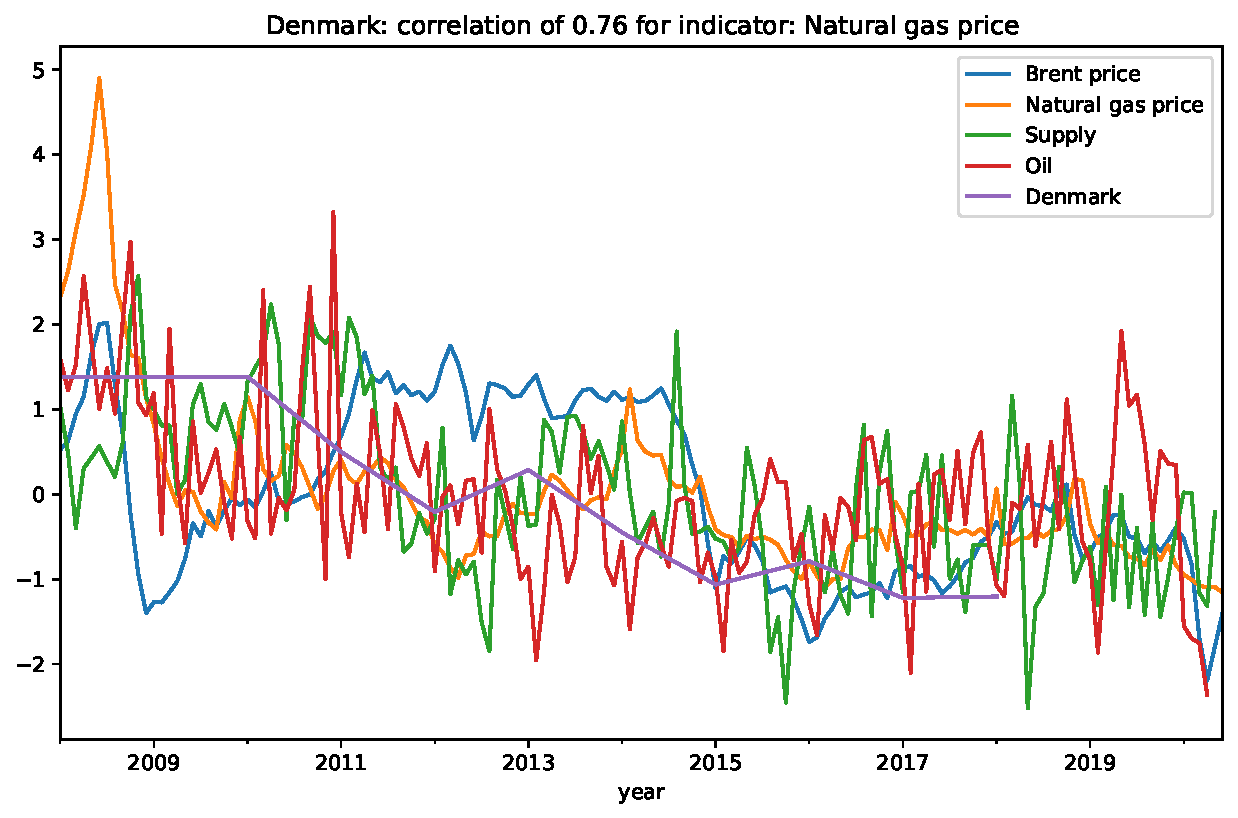
\includegraphics[width=0.5\linewidth]{../power_industry/Denmark_indicators}}
	\subfloat[Portugal]{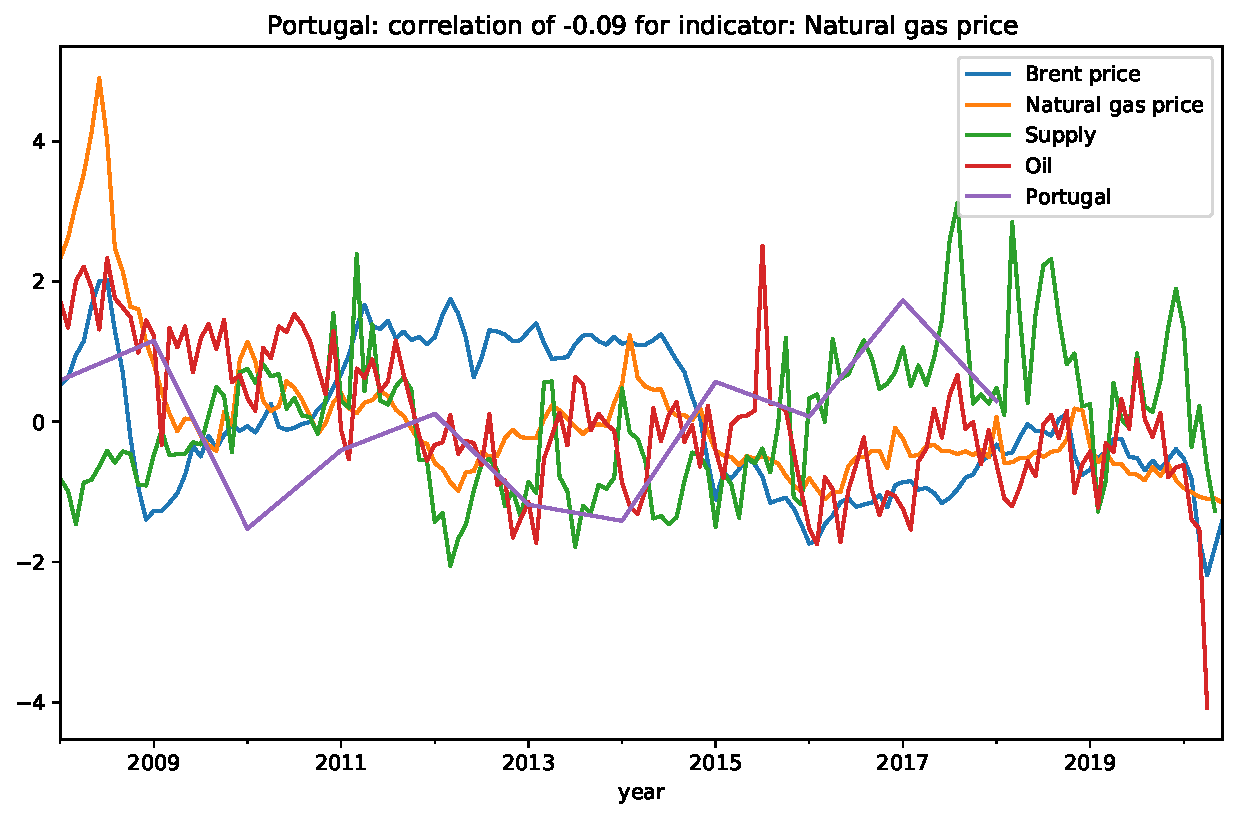
\includegraphics[width=0.5\linewidth]{../power_industry/Portugal_indicators}}
	\caption{Indicators and annual emissions for European countries.}
	\label{fig:indicators_Denmark_Portugal}
\end{figure}

In Table \ref{table:correlation} we can observe the selected indicators and the respective correlation with the emissions for the 8 biggest contributors in emissions.
\begin{table}[h!]
	\centering
	\begin{tabular}{ccc}
		\hline
		Country & Correlation Indicator \& Emissions & Selected Indicator \\
		\hline
		\hline 
		EU & 0.740 & Brent Price \\
		United States & 0.813 & Natural Gas Price \\
		India & -0.272 & Brent Price \\
		China & -0.038 &  Brent Price \\
		Japan &  0.428 & Brent Price \\
		Russia & 0.792 & Brent Price \\
		Canada & 0.785 & Natural Gas Price \\
		Brazil & 0.021 & Brent Price\\
		\hline 
		&& \\
	\end{tabular}
	\caption{Resulting correlations for the biggest contributors}
	\label{table:correlation}  
\end{table}

Once the indicator is selected, SARIMA model is applied per country, allowing us to check if there is a relative change in this indicator and simultaneously to $ CO_2 $ emissions. The results are plotted in Figure \ref{fig:sarima}. 
\begin{figure}[h!]
	\centering
	\subfloat[European Union]{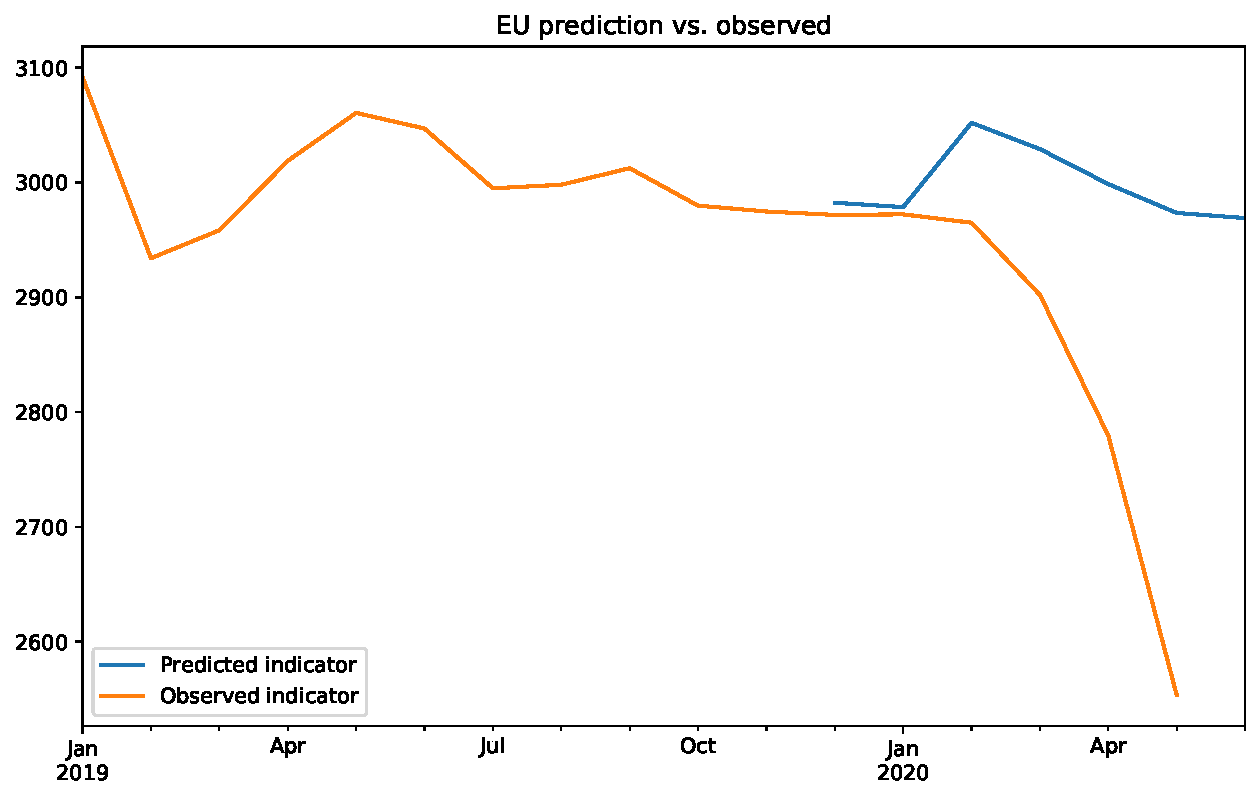
\includegraphics[width=0.4\linewidth]{../power_industry/EU_prediction}}
	\subfloat[United States]{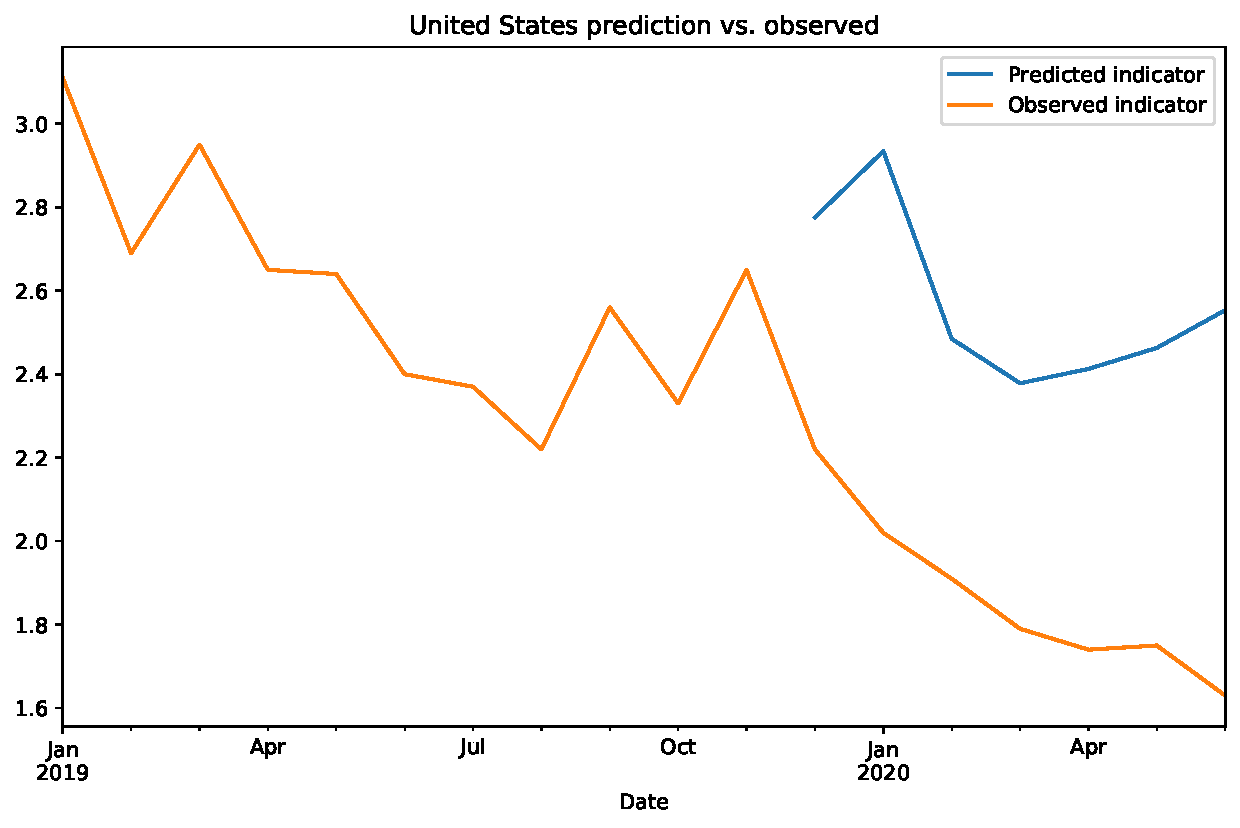
\includegraphics[width=0.4\linewidth]{../power_industry/United States_prediction}} \\
	\subfloat[India]{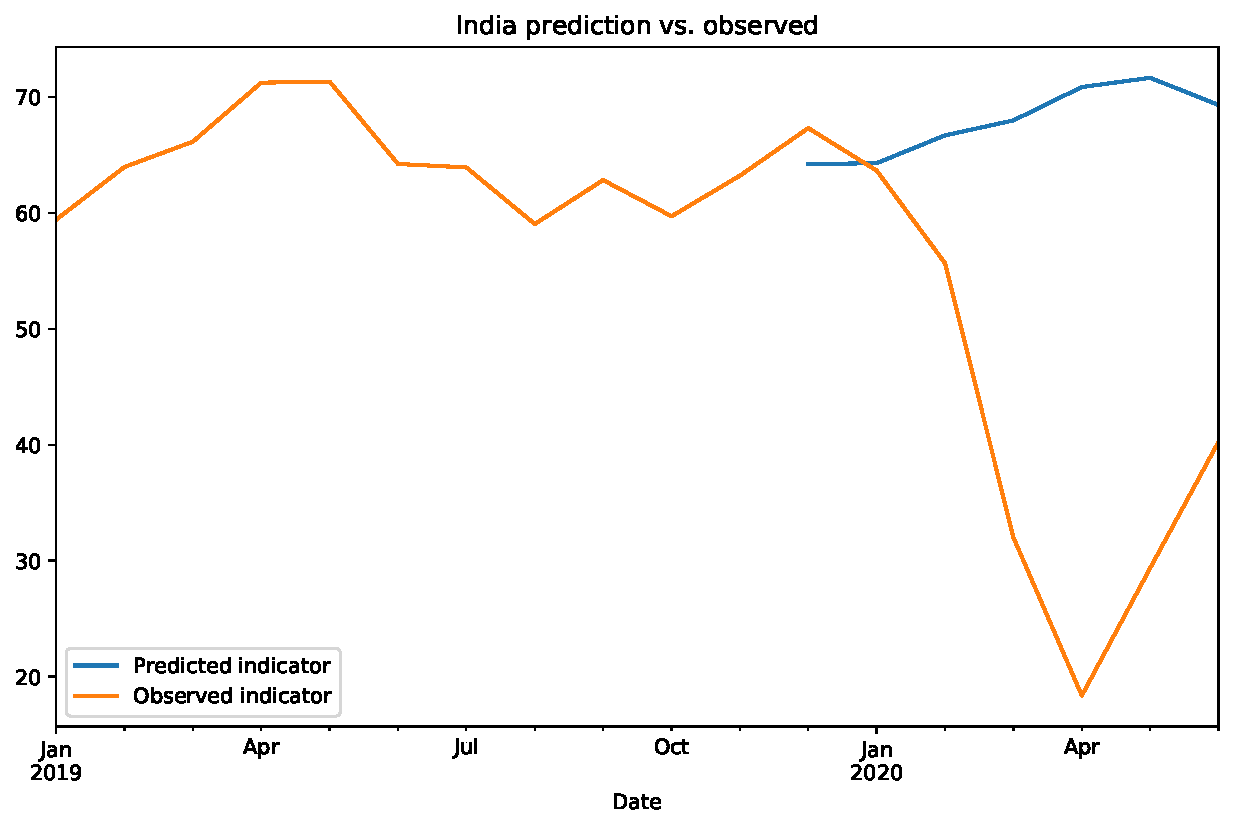
\includegraphics[width=0.4\linewidth]{../power_industry/India_prediction}}
	\subfloat[China]{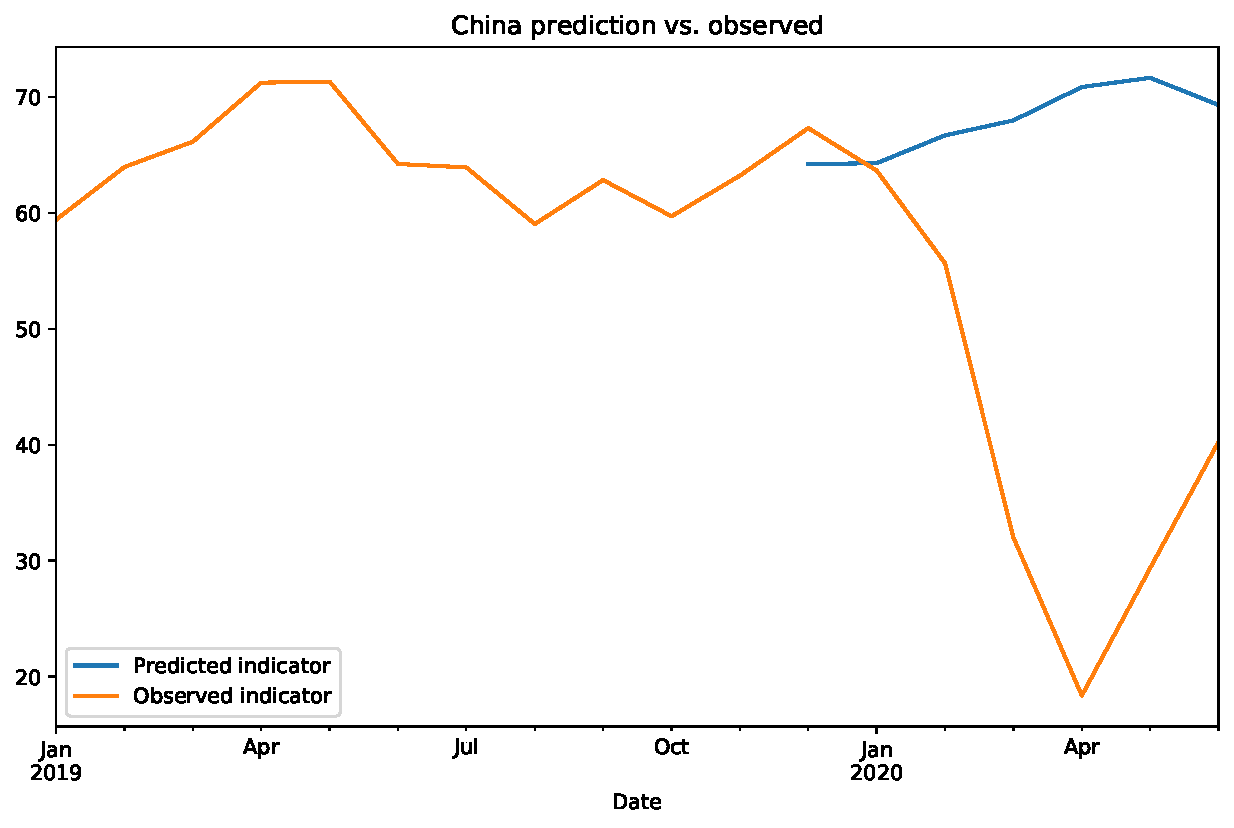
\includegraphics[width=0.4\linewidth]{../power_industry/China_prediction}} \\
	\subfloat[Japan]{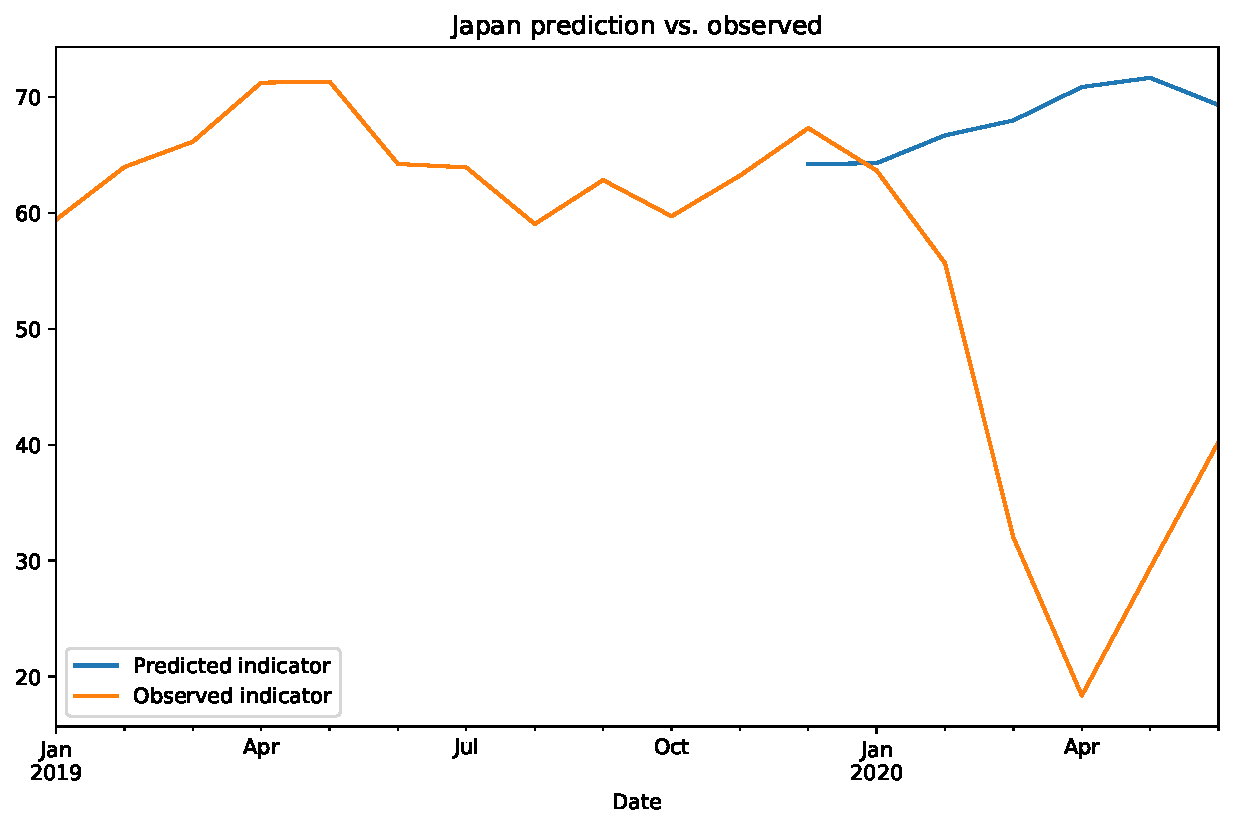
\includegraphics[width=0.4\linewidth]{../power_industry/Japan_prediction}}
	\subfloat[Russia]{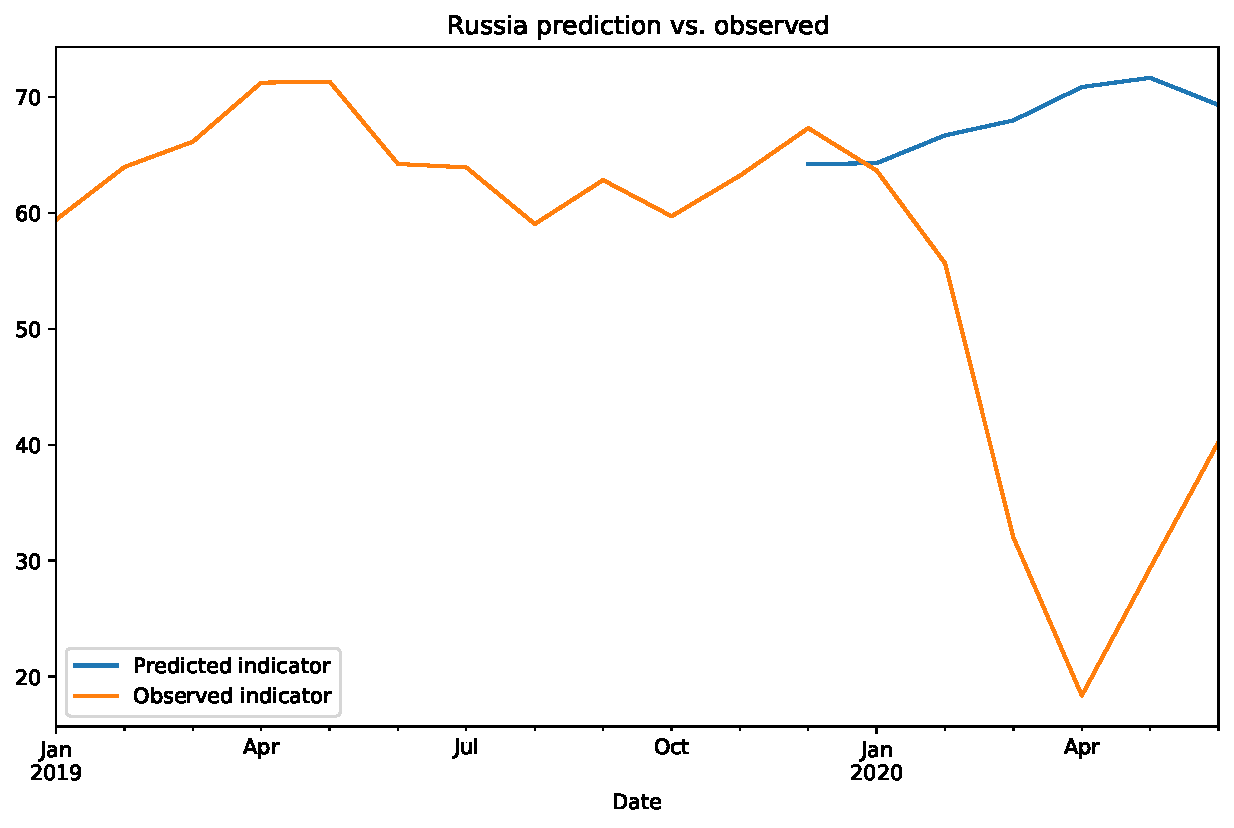
\includegraphics[width=0.4\linewidth]{../power_industry/Russia_prediction}} \\
	\subfloat[Canada]{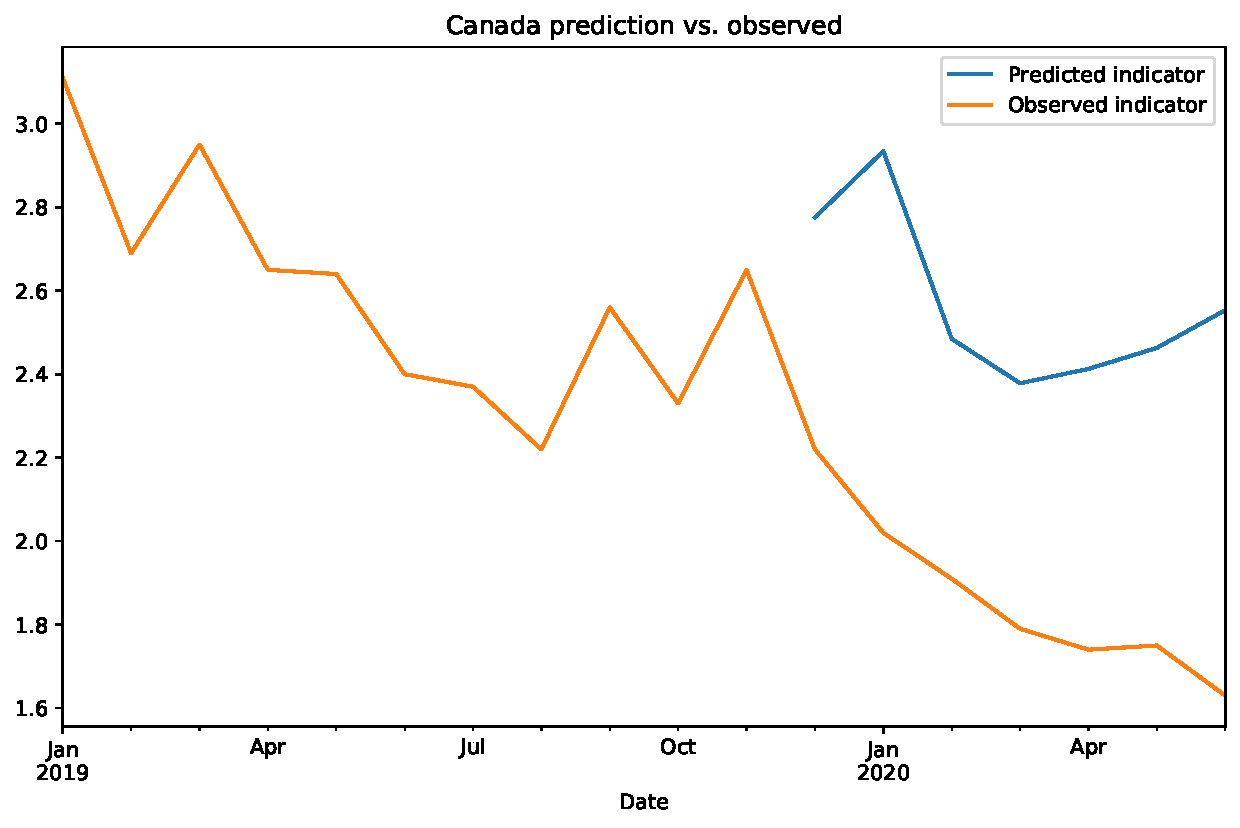
\includegraphics[width=0.4\linewidth]{../power_industry/Canada_prediction}}
	\subfloat[Brazil]{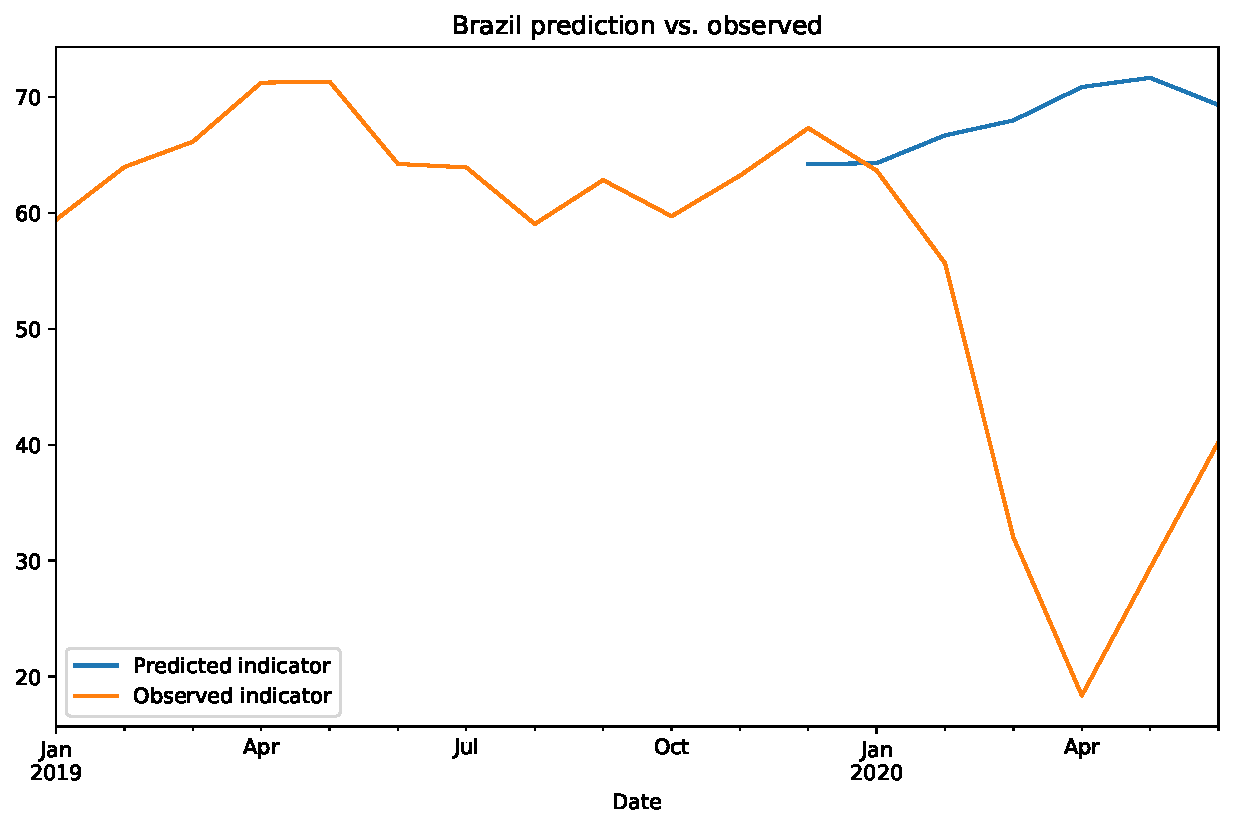
\includegraphics[width=0.4\linewidth]{../power_industry/Brazil_prediction}}
	\caption{Predicted vs real values of selected indicators.}
	\label{fig:sarima}
\end{figure}

In Table \ref{table:change} we show the rate of change for the months we have data. This ratio can be described as:

\begin{equation}
	\text{Rate} = \frac{\text{indicator considering COVID-19}}{\text{indicator without considering COVID-19}} = \frac{\text{actual value of the indicator}}{\text{prediction of the indicator}} 
\end{equation}
\begin{table}[h!]
	\centering
	\begin{tabular}{c|cccccccc}
		\hline
		Country & European Union & United States & India & China & Japan & Russia & Canada & Brazil \\ 
		\hline 
		December, 2019 & 0.996 & 0.800 & 1.048 & 1.048 & 1.048 & 1.048 & 0.800 & 1.048  \\
		January, 2020 & 0.998 & 0.688 & 0.990 & 0.990 & 0.990 & 0.990 & 0.688 & 0.990 \\
		February, 2020 & 0.971 & 0.769 & 0.835 & 0.835 & 0.835 & 0.835 & 0.769 & 0.835 \\
		March, 2020 & 0.958 & 0.752 & 0.471 & 0.471 & 0.471 & 0.471 & 0.752 & 0.471 \\
		April, 2020 & 0.927 & 0.721 & 0.259 & 0.259 & 0.259 & 0.259 & 0.721 & 0.259 \\
		May, 2020 & 0.859 & 0.710 & 0.410 & 0.410 & 0.410 & 0.410 & 0.710 & 0.410 \\
		June, 2020 & \textit{No data} & 0.638 & 0.581 & 0.581 & 0.581 & 0.581 & 0.638 & 0.581 \\
		\hline
	\end{tabular}
	\vspace{1em}
	\caption{Rate of change in the indicator.}
	\label{table:change}  
\end{table}

\paragraph{Conclusion}
Due to the lack of data in emissions of $ CO_2 $, the reliability in our assumptions is based in the correlation with an indicator. Consequently, there are countries which this relation is not very strong and the vector of rate change does not make any sense, since it does not show a reliable situation. 

As mentioned before, non European countries tend to have smaller correlations due to having only two global indicators. In contrast, countries which belong to Europa have four indicators, being two of them unique per country. In results we shown cases with good performance and others which are not optimal, regardless of the region.